\section{Przyszłość - czyli co dalej}
    \tab „Azor” okazał się bardzo zaawansowanym projektem jednak wciąż wymaga wielu ulepszeń i poprawek.
    W tym rozdziale zostaną, krótko omówione możliwe poprawki do zrobienia w przyszłości. Oraz plan dalszego rozwoju projektu.

    \subsection{Do dodania}
        \paragraph{Czujnik cofania\\}
        Jedną z niezbędnych rzeczy jakie powinien posiadać taki robocik jak „Azor” jest czujnik cofania!
        Na dzień pisania tej dokumentacji, użytkownik może kazać „Azorowi” jechać w dowolnym kierunku niezależnie od tego czy na drodze stoi jakaś przeszkoda czy nie.
        \begin{figure}[!h]
            \centering
            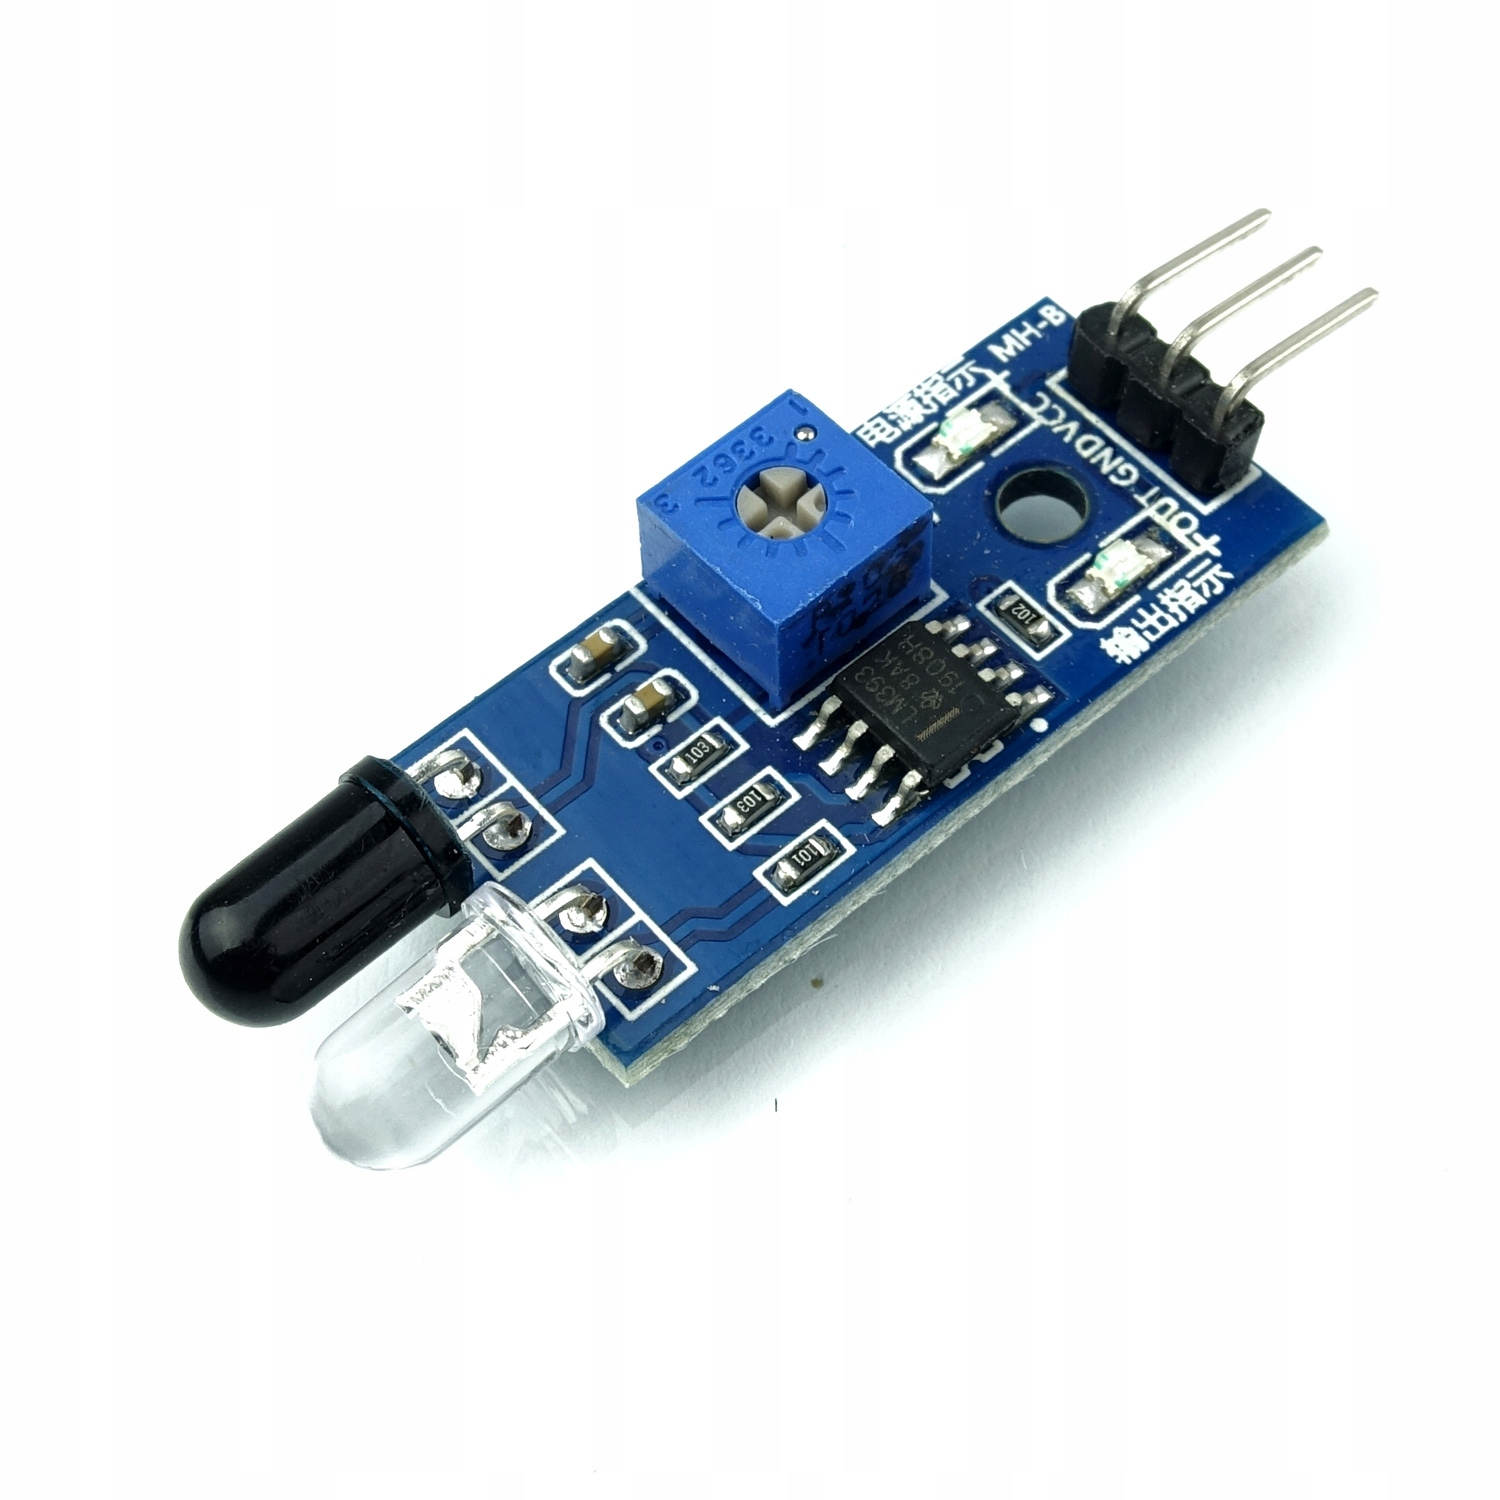
\includegraphics[width = 0.4\textwidth]{Img/czujnik_odleglosci_odbiciowy.jpeg}
            \caption{Przykładowy czujnik cofania}
        \end{figure}


        \paragraph{Wykrywanie przeniesienia\\}
        Następną w kolejności rzeczą do dodania, jest możliwość wykrycia czy „Azor” nie został przeniesiony.
        Dość prosto można wykonać tę operację na akcelerometrze. 
        W momencie wykrycia przyspieszenia w niedozwolonym momencie można wysyłać sygnał przerwania, które będzie zarówno rejestrować wartość przyspieszenia jak i również rozpoczynać pomiar czasu.
        Następnie zgodnie ze wzorem:
        \begin{align}
            \int\limits_0^t a_xt\ dt = x
        \end{align}
        Wyznaczając tę wartość dla osi x oraz y można wyznaczyć przeniesienie „Azora”.

    \newpage
    \subsection{Do poprawy}
        \paragraph{Mikrokontroler\\}
        Pierwszą i najważniejszą rzeczą do wymiany w „Azorze” jest procesor sterujący.
        W tym momencie, jednostką sterującą jest 8-bitowa ATmega328P, która o ile w znaczymy stopniu spełnia zadanie w bardzie złożonej matematyce zaczyna zawodzić.
        Zdecydowanie lepszym rozwiązaniem było by wykorzystanie jakiegoś kontrolera 32-bitowego na przykład STM32 albo dużo tańszego ESP32 lub Seeeduino.

        \paragraph{Silniki i rozłożenie masy\\}
        Aktualnie wykorzystywanymi silnikami są „żółte silniki modelarskie na 6V” i są zdecydowanie za słabe.
        \begin{figure}[!h]
            \centering
            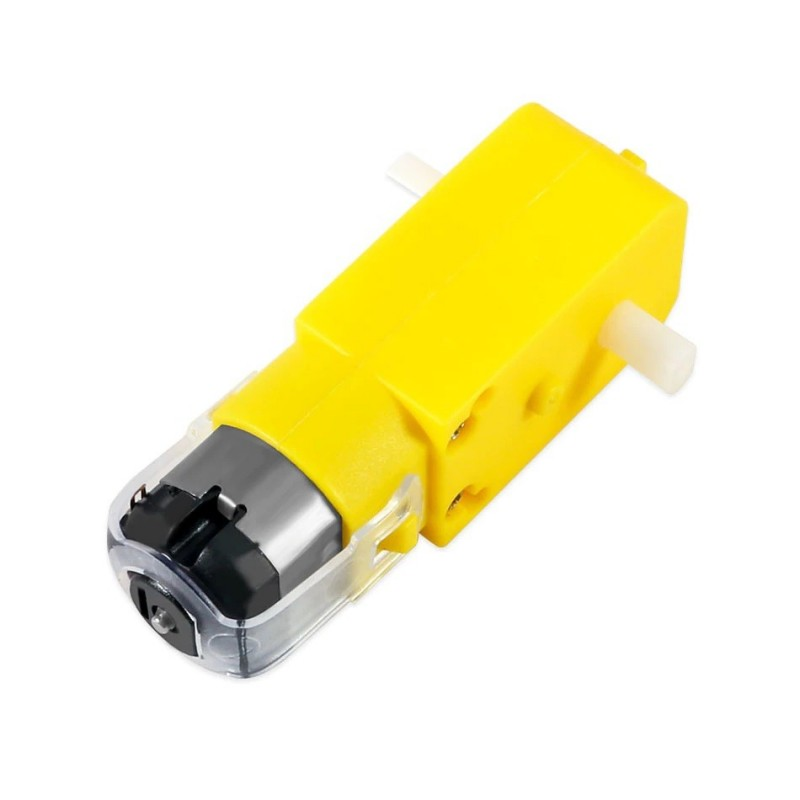
\includegraphics[width = 0.2\textwidth]{Img/silnik.jpg}
            \caption{Silnik uniwersalny z przekładnią}
        \end{figure}
        
        Dodatkową wadą aktualnej konstrukcji jest nierównomierne rozłożenie masy, przez co „Azor” ma tendencję do skręcanie w lewo.